\section{Project report}
In this section i'm going to 
As the project of this course i chose to re-implement some of the tecniques studied during the lectures in another framework based on opitx an API distribuited by NVIDIA which uses parallelization to reduce the rendering times.\\\\
I decided to follow the project initiator to make this project, so the first thing i did was building the framework with Cmake by following the procedure that was written in the project initiator. 
If we run it we get a rendering of a cow that can be seen in figure \ref{fig:cow}.
\begin{figure}[H]
	\centering
	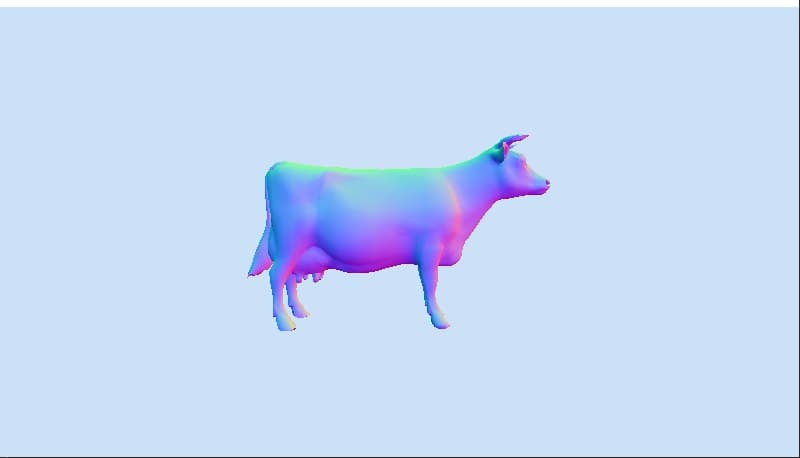
\includegraphics[scale=\imagescale]{images/project/1}
	\caption{}
	\label{fig:cow}
\end{figure}
Since we prefer using the famous stanford bunny for our tests we load this model instead.
\begin{figure}[H]
	\centering
	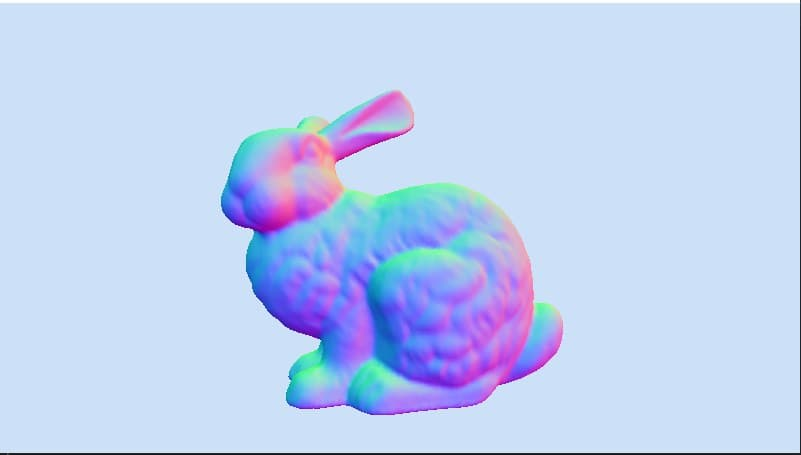
\includegraphics[scale=\imagescale]{images/project/2}
	\caption{}
	\label{fig:bunny}
\end{figure}
Now we implement directional lighting by implementing the directional\_shading function inside the file contained directional\_shader.cu. The result can be seen in figure \ref{fig:directional_shadow}.
\begin{lstlisting}
RT_PROGRAM void directional_shader() 
{ 
	const float3& emission = Ka;
	const float3& rho_d = Kd;
	float3 normal = normalize(rtTransformNormal(RT_OBJECT_TO_WORLD, shading_normal)); 
	float3 ffnormal = faceforward(normal, -ray.direction, normal); 
	float3 color=make_float3(0,0,0);
	
	for(int i=0;i<lights.size();i++){
		color=color+(rho_d/3.14)*lights[i].emission*
			dot(lights[i].direction,ffnormal);
	}
	
	prd_radiance.result = color + emission; 
}
\end{lstlisting}

\begin{figure}[H]
	\centering
	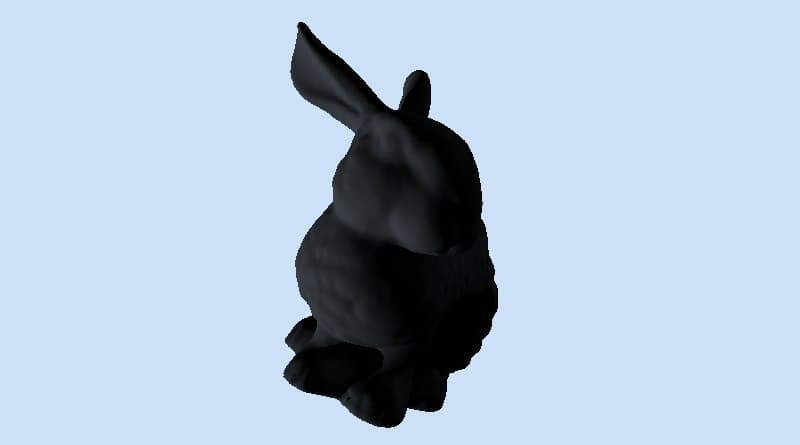
\includegraphics[scale=\imagescale]{images/project/3}
	\caption{Stanford bunny with directional shading}
	\label{fig:directional_shadow}
\end{figure}
Now we add shadows by implementing the function shadow\_shader contained in the file shadow\_shader.cu. The result can be seen in figure \ref{fig:shadow_shading}.
\begin{lstlisting}
RT_PROGRAM void shadow_shader() 
{ 
	#ifdef INDIRECT
	if(prd_radiance.depth > max_depth)
	{
		prd_radiance.result = make_float3(0.0f);
		return;
	}
	#endif
	float3 hit_pos = ray.origin + t_hit * ray.direction;
	float3 normal = normalize(rtTransformNormal(RT_OBJECT_TO_WORLD, shading_normal)); 
	float3 ffnormal = faceforward(normal, -ray.direction, normal); 
	const float3& emission = prd_radiance.emit ? Ka : make_float3(0.0f);
	const float3& rho_d = Kd;
	
	
	float3 color=make_float3(0,0,0);
	for(int i=0;i<lights.size();i++){
		Ray r=make_Ray(hit_pos,lights[i].direction,0,
			scene_epsilon,t_hit-scene_epsilon);
		PerRayData_radiance prd;
		rtTrace(top_shadower,r,prd);
		color=color+(rho_d/3.14)*prd.result*dot(lights[i].direction,ffnormal);
	}
	
	#ifdef INDIRECT
	// Indirect illumination
	uint& t = prd_radiance.seed;
	#endif
	
	prd_radiance.result = color + emission;
}
\end{lstlisting}

\begin{figure}[H]
	\centering
	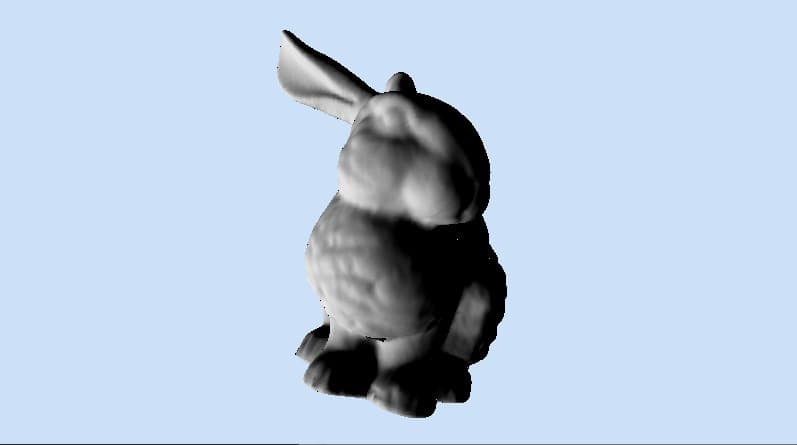
\includegraphics[scale=\imagescale]{images/project/4}
	\caption{Stanford bunny with shadow shading}
	\label{fig:shadow_shading}
\end{figure}
Now we load the cornell box along with the cornell blocks. Since the cornell box has an area light so we have to implement the appropiate shader.\\
Before implementing the area light shader we have to implement the sample\_center function first.
\begin{lstlisting}
__device__ __inline__ void sample_center(const float3& pos, float3& dir, float3& L, float& dist)
{
	float3 light_pos=make_float3(0.0f);
	
	for (int i = 0; i < light_verts.size(); i++) {
		light_pos = light_pos+light_verts[i];
	}
	light_pos = light_pos / light_verts.size();
	
	L = make_float3(0.0f);
	dir = normalize(light_pos - pos);
	dist = length(dir);
	
	float3 avg_normal = make_float3(0.0f);
	for (int i = 0; i < light_idxs.size(); i++) {
		float3 face_normal = normalize(light_norms[light_idxs[i].x] + light_norms[light_idxs[i].y] + light_norms[light_idxs[i].z]);
		avg_normal = face_normal + avg_normal;
		float3 a = light_verts[light_idxs[i].x];
		float3 b = light_verts[light_idxs[i].y];
		float3 c = light_verts[light_idxs[i].z];
		float face_area = (a.x*(b.y - c.y) + b.x*(c.y - a.y) + c.x*(a.y - b.y))/2;
		L = L + dot(-dir, face_normal)*light_emission*face_area;
	}
	avg_normal = avg_normal / light_idxs.size();
}
\end{lstlisting}
Now we can implement the area light shader which is basically only lambertian shading. The result can be seen in figure \ref{fig:area_light}.
\begin{lstlisting}
RT_PROGRAM void arealight_shader() 
{
	#ifdef INDIRECT
	if(prd_radiance.depth > max_depth)
	{
		prd_radiance.result = make_float3(0.0f);
		return;
	}
	#endif
	float3 hit_pos = ray.origin + t_hit * ray.direction;
	float3 normal = normalize(rtTransformNormal(RT_OBJECT_TO_WORLD, shading_normal)); 
	float3 ffnormal = faceforward(normal, -ray.direction, normal); 
	const float3& rho_d = Kd;
	uint& t = prd_radiance.seed;
	float3 color = prd_radiance.emit ? Ka : make_float3(0.0f);
	
	// Direct illumination
	float3 w_i;
	float3 L_e;
	float dist;
	sample_center(hit_pos, w_i, L_e, dist);

	
	Ray r=make_Ray(hit_pos,w_i,0,scene_epsilon,t_hit-scene_epsilon);
	PerRayData_radiance prd;
	rtTrace(top_shadower,r,prd);
	color=color+(rho_d/3.14)*prd.result*dot(w_i,ffnormal);
	
	//color+=rho_d;
	#ifdef INDIRECT
	// Indirect illumination
	#endif
	
	prd_radiance.result = color; 
}
\end{lstlisting}
As we can see from figure \ref{fig:area_light} the area light gets rendered correctly but the rest of the room doesn't seem to be rendered with the correct lighting.\\
Despite the multiple hours i spent trying fixing the problem i didn't manage to do it. However i think that the problem is in the shader and that the sampling function is implemented correctly.
\begin{figure}[H]
	\centering
	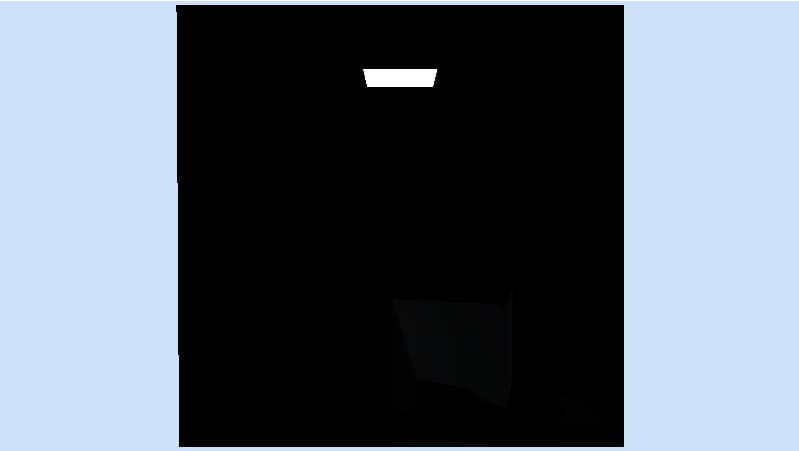
\includegraphics[scale=\imagescale]{images/project/6}
	\caption{Cornell box and cornell blocks}
	\label{fig:area_light}
\end{figure}
If we load a pair of spheres instead of the CornellBoxes we can see that a second area light appears that previously was covered by the boxes. Such rendering can bee seen in figure \ref{fig:cornell_spheres}. We can notice that some weird shadows are being casted on the surfaces of the box, this is happens probably for the same reasons listed before.
\begin{figure}[H]
	\centering
	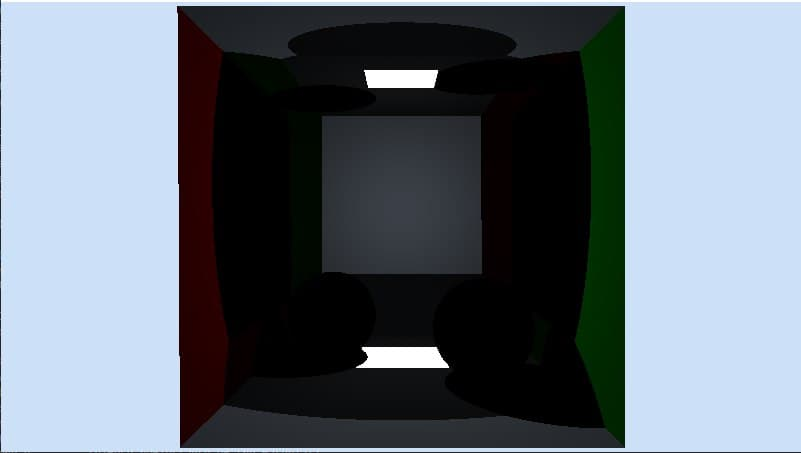
\includegraphics[scale=\imagescale]{images/project/7}
	\caption{Cornell box with spheres}
	\label{fig:cornell_spheres}
\end{figure}
The two spheres that can be seen in figure \ref{fig:cornell_spheres} are made of a transparent and mirror-like material. Since the shaders for this materials are not implemented yet for now they appear completly black. So to render them correcly we have to implement the appropiate shaders.\\
We start by implementing the mirror\_shader contained in the file mirror\_shader.cu
\begin{lstlisting}
RT_PROGRAM void mirror_shader()
{
	if(prd_radiance.depth > max_depth)
	{
		prd_radiance.result = make_float3(0.0f);
		return;
	}
	
	float3 hit_pos = ray.origin + t_hit * ray.direction;
	float3 normal = normalize(rtTransformNormal(RT_OBJECT_TO_WORLD, shading_normal));
	
	prd_radiance.result = make_float3(0.0f);
	if(prd_radiance.depth<=max_depth){
		float3 reflected_dir=reflect(ray.direction,shading_normal);
		PerRayData_radiance prd;
		float3 hit_pos=ray.direction*t_hit;
		Ray r=make_Ray(hit_pos,reflected_dir,0,scene_epsilon,RT_DEFAULT_MAX);
		rtTrace(top_object,r,prd_radiance);
		prd_radiance.depth+=1;
	}
}
\end{lstlisting}

\begin{figure}[H]
	\centering
	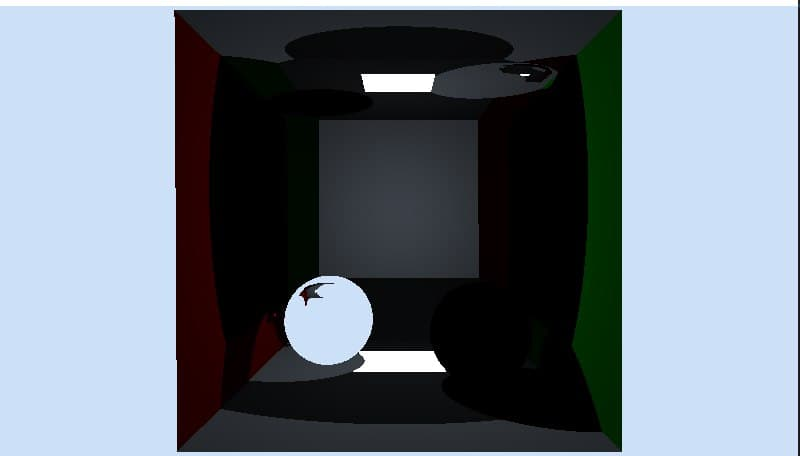
\includegraphics[scale=\imagescale]{images/project/9}
	\caption{Mirror sphere}
	\label{fig:mirror_ball}
\end{figure}
And then we do the same for the transparent\_shader function contained in the transparent\_shader.cu file.
\begin{lstlisting}
RT_PROGRAM void transparent_shader()
{
	if(prd_radiance.depth > max_depth)
	{
		prd_radiance.result = make_float3(0.0f);
		return;
	}
	
	float3 hit_pos = ray.origin + t_hit * ray.direction;
	float3 normal = normalize(rtTransformNormal(RT_OBJECT_TO_WORLD, shading_normal));
	float3 result = make_float3(0.0f);
	
	result=make_float3(0.0f);
	PerRayData_radiance out_prd;
	out_prd.depth=prd_radiance.depth-1;
	if(prd_radiance.depth<=max_depth){
		float3 reflected_dir=reflect(ray.direction,shading_normal);
		PerRayData_radiance prd;
		float3 hit_pos=ray.direction*t_hit;
		Ray reflect_r=make_Ray(hit_pos,reflected_dir,0,
			scene_epsilon,RT_DEFAULT_MAX);
		rtTrace(top_object,reflect_r,prd_radiance);
		prd_radiance.depth+=1;
		
		float3 refract_dir;
		bool refraction=refract(refract_dir,ray.direction,shading_normal,ior);
		Ray refract_r=make_Ray(hit_pos,refract_dir,0,scene_epsilon,RT_DEFAULT_MAX);
		rtTrace(top_object,reflect_r,prd_radiance);
		
		if(refraction){
			rtTrace(top_object,reflect_r,out_prd);
			out_prd.depth+=1;
		}	  
		
		
		float cos_theta=dot(ray.direction,shading_normal);
	}
	result=prd_radiance.result+out_prd.result;
	prd_radiance.result = result;
}
\end{lstlisting}

\begin{figure}[H]
	\centering
	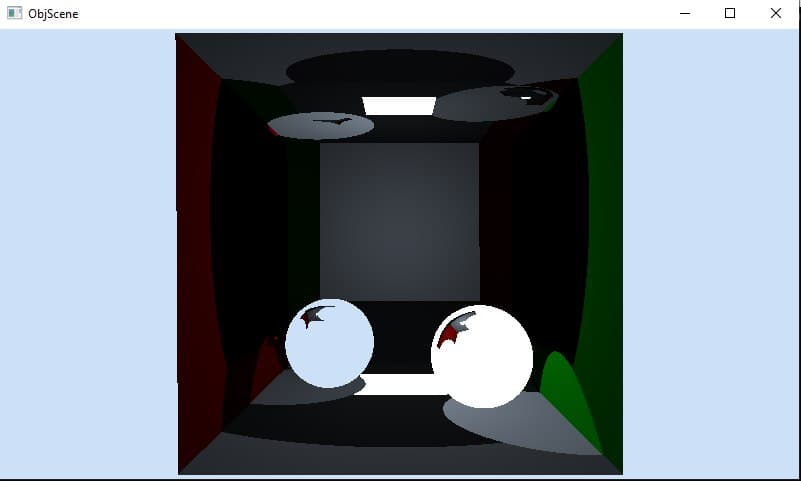
\includegraphics[scale=\imagescale]{images/project/10}
	\caption{Transparent sphere}
	\label{fig:transparent_sphere}
\end{figure}